\section{STM32-Based Field-Oriented Control Motor Drive}
\label{sec:foc}

This section presents the design and implementation of a high-performance motor controller based on Field-Oriented Control (FOC).

\subsection{Choice of FOC Over Trapezoidal Commutation}

Table~\ref{tab:foc_vs_trap} summarizes the key differences between the two commutation strategies, based on the literature reviewed in Section~\ref{sec:relatedwork}.

\begin{table}[htbp]
\caption{Comparison between FOC and trapezoidal (six-step) commutation}
\label{tab:foc_vs_trap}
\centering
\begin{tabular}{lcc}
\toprule
\textbf{Criterion} & \textbf{FOC} & \textbf{Six-Step} \\
\midrule
Torque ripple (at 500 rpm) & \SI{18.4}{\percent} & \SI{35.7}{\percent} \\
Low-load efficiency & High & Moderate \\
High-speed switching loss & Higher & Lower \\
Position sensor requirement & Encoder (high resolution) & Hall sensors \\
Implementation complexity & High & Low \\
Hardware cost & Higher & Lower \\
Dynamic response & Fast & Standard \\
\bottomrule
\end{tabular}
\end{table}

For our cargo bike application, rider comfort and smooth torque delivery are priorities. FOC was therefore selected for the high-performance controller, while a separate low-tech six-step board (Section~\ref{sec:sixstep}) was developed for repairability.

\subsection{Base Design: Cheap FOCer-2 Project}

The starting point was the open-source \textit{Cheap FOCer-2} project, which provides a complete KiCad design for a VESC-compatible board based on an STM32F405 microcontroller. This design includes:
\begin{itemize}
    \item A three-phase MOSFET full-bridge power stage.
    \item Gate drivers with built-in dead-time insertion.
    \item Shunt resistors for phase current sensing.
    \item USB and CAN interfaces.
    \item An expansion header for encoder or Hall sensors.
\end{itemize}

The existing KiCad schematic and layout were used as the baseline for our adaptations.

\subsection{Integration of the Rocacher FOC Tile}

Mr. Rocacher provided the Kicad schematic of a ready-to-use FOC tile based on an STM32L476 microcontroller.

The initial idea was to make this tile \textit{pluggable} into our carrier board, similar to an Arduino shield. This would allow :
\begin{itemize}
    \item Easy replacement of the computing core without re-soldering.
    \item Modular upgrades of the microcontroller.
    \item Simplified repair and maintenance.
\end{itemize}

However, the Cheap FOCer-2 project was not designed for such modularity. Its routing is dense and highly optimized for a single, non-removable F405 chip. Adapting it to accept an L476 tile while preserving all critical functions (PWM, current sensing, USB communication) proved challenging.

\subsection{Pin Compatibility Verification: L476 vs F405}
Before starting the PCB modifications, a pin compatibility study was carried out between the STM32L476 used on the Rocacher tile and the STM32F405 originally used in the Cheap FOCer-2 design. The objective was to verify that the main functions required by the VESC firmware could still be used after replacing the original microcontroller.

The verification mainly focused on:
\begin{itemize}
    \item Physical pinout compatibility in the LQFP64 package,
    \item PWM timer for Alternate functions,
    \item USB DP/DM pins (PA11/PA12),
    \item Analog inputs for current sensing,
    \item UART communication for BLE integration.
\end{itemize}

During this analysis, three main pin conflicts were identified.

\begin{figure}[!h]

    \centering
    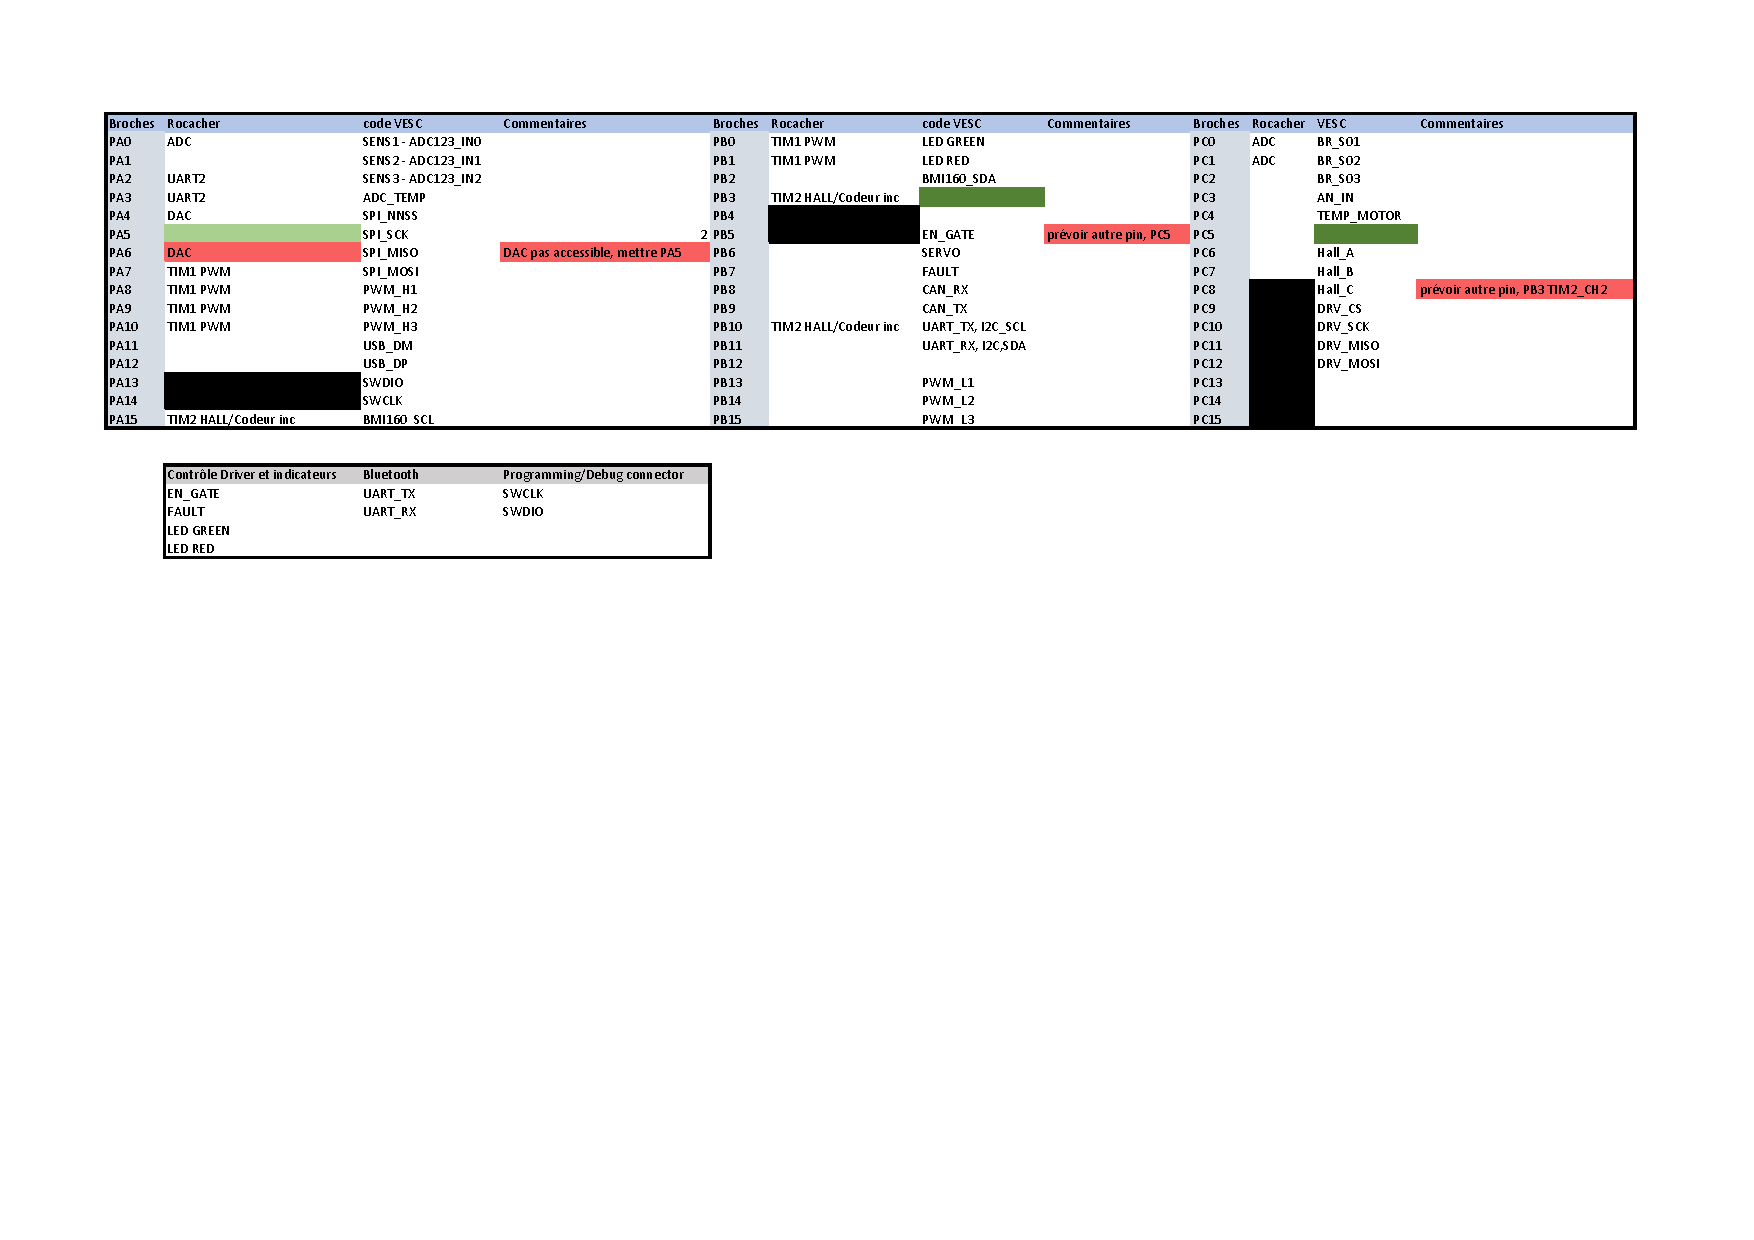
\includegraphics[width=\linewidth]{Figures/CompatibiliteL4F4.pdf}
    \caption{Comparison of F405 and L476 pin configurations}
    
\end{figure}

The first conflict concerned the SPI\_MISO signal on pin PA6. In the original STM32F405 design, this pin is used for SPI communication related to current sensing. On the STM32L476 tile, the same pin is associated with a DAC output, creating a functional conflict. To solve this issue, the SPI communication line was remapped to PA5 on the L476, which offers a compatible alternate function.

The second issue concerned the EN\_GATE signal. In the original design, this signal was connected to PB5 on the STM32F405. However, this pin is not accessible on the L476 tile. The signal was therefore moved to PC5, configured as a standard GPIO output.

Finally, Hall sensor C was originally connected to PC8 (TIM8) on the STM32F405. Since this pin is not available on the tile connector, the Hall sensor input was reassigned to PB3 using the TIM2\_CH2 alternate function, which preserves the input capture capability required for Hall sensor decoding.

All other important functions remained compatible between the two microcontrollers, including PWM generation, complementary PWM outputs, encoder inputs, UART, USB, and CAN communication. Some differences between the ADC peripherals of the STM32F405 and STM32L476 still remain and will require firmware adaptations in future work.

\subsection{Schematic Design and KiCad Implementation}

The original Cheap FOCer-2 schematic was modified in KiCad in order to replace the integrated STM32F405 microcontroller with connectors for the Rocacher STM32L476 tile. The objective was to make the control part more modular and easier to replace without modifying the power stage of the board.

The main modifications performed on the schematic were:
\begin{itemize}
    \item Removal of the STM32F405 and its associated passive components.
    \item Addition of two 20-pin headers for the L476 tile connection.
    \item Re-routing of PWM, ADC, USB, and communication signals toward the headers.
\end{itemize}

Special attention was given to the routing of critical control signals, especially the PWM outputs used for motor commutation and the analogue signals used for current sensing.

After the modifications, the schematic was verified using the KiCad Electrical Rule Check (ERC). No electrical errors were detected during this verification step, which validated the consistency of the schematic before starting the PCB routing phase.

\subsection{Routing Challenges and Current Status}

After validating the schematic, the PCB routing phase was started in KiCad. The original Cheap FOCer-2 board uses a very compact layout with dense routing around the STM32F405 microcontroller and the power stage. Integrating connectors for a removable STM32L476 tile introduced several additional routing constraints.

One of the main difficulties was maintaining proper signal routing while keeping enough space for the tile connectors and preserving the integrity of the control signals. Particular attention had to be given to the PWM signals, current sensing traces, and power connections.

Several issues were encountered during the routing process:
\begin{itemize}
    \item Some connector footprints associated with the tile did not appear correctly after importing the schematic into the PCB layout.
    \item The routing of high-current paths, especially the battery and motor phase connections, become more complex due to the additional connectors and required extra vias.
    \item Some Decoupling capacitors had to be repositioned, which could potentially affect switching noise and power
     supply stability.
\end{itemize}

At the current stage of the project, the schematic has been validated and the PCB layout is still under development. Once the routing is completed, the board will be manufactured and tested using the VESC firmware adapted for the STM32L476 tile.
